\documentclass[11pt]{article}
\usepackage[margin=1in]{geometry}
\usepackage[T1]{fontenc}
\usepackage{lmodern}
\usepackage{microtype}
\usepackage{amsmath}
\usepackage{booktabs}
\usepackage{graphicx}
\usepackage{xcolor}
\usepackage[numbers,sort&compress]{natbib}
\usepackage[hidelinks]{hyperref}
\usepackage{CJKutf8}

\newcommand{\zh}[1]{\begin{CJK}{UTF8}{gbsn}#1\end{CJK}}
\newcommand{\todo}[1]{\textcolor{red}{[TODO: #1]}}

\title{Adapting a Latent Audio Diffusion Model to Historical Guqin Recordings:\\
A Listening-Driven Case Study}
\author{Huanchen Cai\thanks{\todo{affiliation and contact e-mail}}}
\date{October 2026}

\begin{document}
\maketitle

\begin{abstract}
We report a small-data case study in adapting a pretrained latent audio diffusion model to the guqin, the
seven-string Chinese zither, with the long-term goal of an ``AI radio'' that plays guqin-style music without end.
From a library of historical recordings we curate 412 solo performances (42.5\,h, 61 performers) and split them
by composition. We fine-tune a rank-16 DoRA adapter on Stable Audio~3 Medium using its continuous SAME-L latents,
continuation-oriented masking, captions combining researched notes on each piece with mood tags and an
automatically estimated pentatonic mode, and random-length crops, and we stop training when held-out
validation loss stops improving. Seven blind listening studies by one expert listener guide every decision.
The final adapter (pass~14 of 17) received the highest mean rating for continuing unseen pieces (3.9/5 versus
3.4 for the best earlier adapter and 2.8 for an early checkpoint of the same run) and 4.6/5 for generating from
free-written scene descriptions. Equally informative are the failures: a from-scratch autoregressive model over
the same latents produced no recognisable timbre; a signal-level ``friction noise'' measure correlated with the
listener's ``sawing'' complaints in the wrong direction; and a pentatonic-fit measure tracked ratings overall
($\rho=0.52$) but barely within a group of candidates. Chaining continuations for long playback exposed two
mechanical problems, a silent tail on every generated clip and a loudness feedback loop, both of which have simple
fixes. With a single listener and at most ten clips per condition, none of the paired differences is
statistically significant; we present the results as an exploratory record of what helped, what did not, and why.
\end{abstract}

\section{Introduction}

Text-to-music and audio continuation models are trained mostly on Western popular and library music.
The guqin is a poor fit for that prior: its repertoire is largely pentatonic, its expressive vocabulary
lives in left-hand slides and vibrato (\zh{吟猱绰注}) whose passing semitones are idiomatic only in specific places,
and the best-known performances survive mainly as mid-twentieth-century recordings with tape hiss and
limited bandwidth. The amount of usable solo audio is also small---tens of hours, not thousands.

Our practical goal is an ``AI radio'': a system that keeps producing guqin-like music for hours, either continuing
from a recorded opening or following a short textual description of a scene. This report documents how we got
from a general-purpose model to an adapter that a guqin-literate listener rates as convincing, and records the
dead ends along the way, because in a domain this small the negative results are a large part of what was learned.

Our contributions are:
\begin{itemize}
  \item A curation and evaluation protocol for a small historical corpus: expert screening of every recording,
        composition-level splits so that test pieces are never heard in another performer's version, and blind,
        shuffled listening with free-text comments (\S\ref{sec:data}, \S\ref{sec:eval}).
  \item A fine-tuning recipe for Stable Audio~3 Medium~\citep{evans2026stableaudio3} on 42\,h of audio:
        DoRA~\citep{liu2024dora} on the base model with inference on the distilled model, masking weighted towards
        prefix continuation, captions that mix researched notes on each composition with mood tags and an estimated
        pentatonic mode, random-length crops, and early stopping on held-out loss (\S\ref{sec:method}).
  \item Seven listening studies and the decisions they drove, including clear negative results for a
        from-scratch latent language model and for two automatic quality measures (\S\ref{sec:results}).
  \item Two practical failure modes of chained continuation for long playback, with fixes (\S\ref{sec:chain}).
\end{itemize}

\section{Related work}

\paragraph{Latent audio diffusion.} Stable Audio~\citep{evans2024fast} generates variable-length audio by
diffusion in the latent space of an autoencoder, conditioned on text and timing; Stable Audio
Open~\citep{evans2024open} and Stable Audio~3~\citep{evans2026stableaudio3} extend this with open weights,
inpainting and continuation. Long-form generation with latent diffusion~\citep{evans2024longform} shows that
the training window length matters for musical structure. We build directly on Stable Audio~3 Medium and its
continuous SAME-L autoencoder.

\paragraph{Autoregressive music models.} Token-based language models such as MusicGen~\citep{copet2023musicgen}
and streaming systems such as Magenta RealTime~\citep{lyria2025live} generate indefinitely by construction.
Continuous-latent autoregression with a diffusion or flow head~\citep{li2024mar} avoids quantisation, and noise
augmentation of the context reduces error accumulation~\citep{pasini2024continuous}. We test a small model of this
kind trained from scratch (\S\ref{sec:latentlm}).

\paragraph{Parameter-efficient adaptation and small data.} LoRA~\citep{hu2021lora} and DoRA~\citep{liu2024dora}
adapt large models with few trainable parameters. For data-constrained training, repeating data for a few
epochs is nearly as useful as fresh data~\citep{muennighoff2023scaling}, which motivates our multi-pass schedule
with early stopping.

\paragraph{Guqin and evaluation.} Prior guqin MIR work analyses mode and playing technique from historical
recordings~\citep{huang2020guqin}. For generated music, replication of training data is a central
concern~\citep{batlleroca2024replication}; we keep evaluation pieces out of training at the composition level.

\section{Data}\label{sec:data}

\paragraph{Source and screening.} The source is a private library of 638 historical guqin recordings
(44.1\,kHz, 16-bit stereo CD transfers). Every candidate was screened by the author, a guqin-literate
listener, through a whole-track listening page; recordings were excluded for audible noise floors, ensembles
or non-guqin instruments, and voice. The result is \textbf{412 solo recordings by 61 performers, 42.5\,h}, with
108 distinct titles after normalising numbered variants (a few titles are alternative names of the same piece). Performer coverage is
uneven: the five most represented performers account for about 40\% of the duration.

\paragraph{Splits.} We split by composition rather than by performer, so that no version of a test composition is
heard in training: 329 recordings for training, 42 for validation and 41 for test. Each recording is cut into
aligned windows of the model's native length (59.9\,s, 2{,}641{,}920 samples) that together cover the whole
performance, giving 2{,}764 windows (2{,}217/276/271); nine windows of pure digital silence are dropped. The
final run trains on training and test recordings together (370 recordings) and keeps the 42 validation
recordings out for early stopping and listening.

\paragraph{Captions.} For each composition we compiled a short narrative from published notes on the piece
(e.g.\ \textit{Liushui}, Boya and his true listener Ziqi; \textit{Guangling San}, Nie Zheng's revenge and Ji
Kang's last performance), assigned two to five tags from a closed vocabulary of 37 moods and scenes (e.g.\
\textit{calm, lonely, vast, reclusive, autumn, river, frontier desert}), and recorded our confidence: 55 notes are
well sourced, 31 partly, and 22 inferred from the title. A pentatonic mode (the \emph{gong} pitch and its five
notes) is estimated automatically for every window from a tuning-corrected pitch-class histogram. Captions are
written in English with the Chinese text appended and never exceed 160 tokens of the 256-token encoder limit.

\section{Method}\label{sec:method}

\paragraph{Model.} Stable Audio~3 Medium~\citep{evans2026stableaudio3} is a diffusion transformer over SAME-L
latents (256 dimensions at about 10.8 frames per second) conditioned on T5Gemma text embeddings and on an
inpainting mask. Following the released recipe, we train a rank-16 DoRA adapter (21.6\,M trainable parameters)
on the \emph{base} model and apply it to the step-distilled \emph{Medium} model at inference (8 sampling steps).
All latents are pre-encoded once.

\paragraph{Objective and masking.} Training uses the model's rectified-flow objective~\citep{liu2022rectified}
with its inpainting conditioning. We change the masking mixture from the default
10/80/10 (random spans / fully masked / prefix continuation) to 10/30/60, so that most training examples
resemble our main use, continuing a given opening.

\paragraph{Text.} Each window receives one caption style by a stable hash: 40\% tags + mode, 40\% narrative +
tags + mode, 20\% narrative only; the trainer additionally drops 10\% of captions for classifier-free use.

\paragraph{Crops and schedule.} Each sample keeps a random span of 20--60\,s at a random start inside its window,
padded with the silence latent and with the timing condition set to the kept length. One training pass is
2{,}500 steps at batch size 1 (about one epoch), learning rate $10^{-4}$, AdamW. After each pass we compute the
model's validation loss at five fixed noise levels on all 276 validation windows and stop when three
consecutive passes fail to improve on the best. Checkpoints every 500 steps make the run resumable after
interruptions.

\paragraph{Inference.} Continuation keeps a 10\,s opening and generates the next 25\,s; text-only generation
produces 35\,s from a description. For long playback we chain continuations (\S\ref{sec:chain}).

\section{Evaluation protocol}\label{sec:eval}

All listening was done by the author, who has extensive experience with the guqin repertoire, on local
web pages in a fixed format: candidates for the same opening and seed are shuffled and unlabeled; each clip
gets an overall score from 1 to 5, optional issue tags (e.g.\ \emph{too many semitones}, \emph{sawing/metallic
noise}, \emph{not guqin-like}, \emph{no melody}, \emph{abrupt seam}) and free-text comments; the mapping is
revealed only after rating. Openings come from compositions the compared models did not train on, with each
study using different performers and pieces where possible. For paired comparisons we report exact two-sided
sign-flip permutation tests over openings and percentile bootstrap intervals; with eight or fewer pairs these
tests have little power and we treat them as descriptive.

\section{Results}\label{sec:results}

Table~\ref{tab:studies} summarises the seven studies. Scores are means over clips; $n$ is clips per condition.

\begin{table}[t]
\centering
\small
\begin{tabular}{@{}p{3.3cm}p{6.4cm}rp{2.7cm}@{}}
\toprule
Study & Condition & $n$ & Mean \\
\midrule
R1 masking (329 vs 412) & default mask / continuation mask / 412, cont.\ mask & 8 & 2.88 / 2.62 / 3.38 \\
R2 inference settings & strength 1.0 / 0.7 / LoRA early steps only & 9--10 & 3.56 / 3.60 / 3.67 \\
 & base model, 50 steps / earlier 222-clip adapter & 10 & 2.70 / 3.10 \\
R3 captions (continuation) & no text in training / no prompt / matching / opposite tags & 9 & 3.89 / 3.56 / 4.00 / 4.00 \\
R3 captions (text only) & adapter without / with caption training & 5 & 2.00 / 3.80 \\
R4 latent LM & from-scratch latent LM / SA3 adapter & 11 / 6 & 1.00 / 2.00 \\
R5 longer training & 1 pass / 3 passes + tags / 3 passes + tags + mode & 8 & 3.75 / 3.75 / 4.12 \\
R6 narrative captions & pass 2 / adapter C (R5) & 7 / 8 & 3.00 / 3.50 \\
R7 final & pass 14 / pass 2 / adapter C & 8 & \textbf{3.88} / 2.75 / 3.38 \\
R7 final (scenes) & pass 14 / pass 2 & 5 & \textbf{4.60} / 3.60 \\
\bottomrule
\end{tabular}
\caption{Overview of the listening studies (scores 1--5, single expert listener). In R1 the 412-recording adapter had seen the validation compositions; all other comparisons use openings unseen by every compared model, except R2 (see \S\ref{sec:limits}).}
\label{tab:studies}
\end{table}

\paragraph{Seed and opening dominate.} In R1 the two seeds differed by 1.6 points on average (2.17 vs 3.75),
more than any model difference; in R2 the mean per opening-and-seed group ranged from 1.0 to 4.75 while
inference settings moved the mean by at most 0.1 (except the base model). The same semitone often appeared at the
same second in all candidates sharing an opening and seed. This variance motivates generating several takes and
selecting, and it is why per-condition means over a handful of clips must be read cautiously.

\paragraph{Inference settings.} Lowering adapter strength or restricting the adapter to early denoising steps
made no difference. Using the base model with 50 steps---the configuration matching training---was clearly
worse (2.70, five scores of 1, comments about extra instruments), confirming that the distilled model is the
better renderer.

\paragraph{Text conditioning.} Training with mood tags left continuation unchanged (matching and deliberately
opposite tags both scored 4.0: the opening dominates), but improved generation from text alone from 2.0 to 3.8
($p=0.06$, $n=5$).

\paragraph{Training length.} On the 329-piece split, held-out loss decreased monotonically over three passes
(0.5387 base, 0.5351, 0.5343, 0.5337) with no sign of overfitting; captions and mode text did not change the loss.
In the final run (Figure~\ref{fig:val}) the loss fell from 0.6020 to a minimum of 0.5950 at pass~14 and rose
over the next three passes, triggering early stopping. The pass-14 adapter improved continuation over the
pass-2 checkpoint of the same run (3.88 vs 2.75, $p=0.16$) and over adapter~C (3.38, $p=0.63$), and received no
``sawing'' tags against three for pass~2. Bootstrap 95\% intervals are wide ([2.75, 4.75] for pass~14).
For scene descriptions written after training, pass~14 scored 4.6 against 3.6 ($p=0.31$); one take was singled
out by the listener as exceptional.

\begin{figure}[t]
\centering
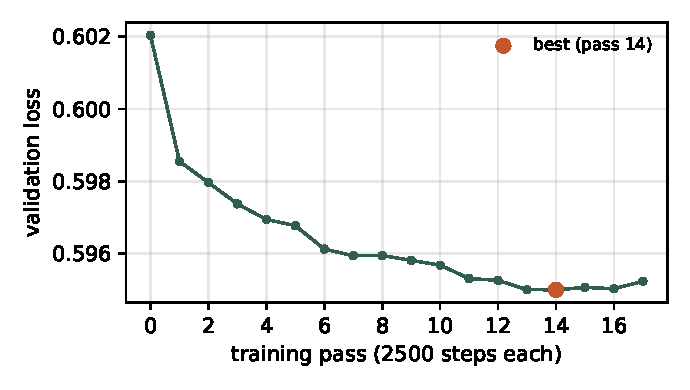
\includegraphics[width=0.6\linewidth]{generated/val_loss.pdf}
\caption{Validation loss per training pass of the final run (276 held-out windows, five fixed noise levels).}
\label{fig:val}
\end{figure}

\subsection{Negative result: a from-scratch latent language model}\label{sec:latentlm}

We trained a causal transformer (8 layers, width 512) with a flow-matching MLP head that predicts the next
SAME-L frame, with context noise augmentation~\citep{pasini2024continuous} (72\,M parameters, 1.42\,M training
frames). Validation loss reached its minimum at 10k steps and rose by 8\% by 40k steps (Figure~\ref{fig:lm}).
Every one of its 11 clips received the lowest score, including endless and unconditioned generation, with
comments such as ``no timbre at all''; independently sampled frames left the region the decoder renders as
guqin. The same openings continued by the SA3 adapter scored 2.0. At this data scale a frame-level autoregressive
model over continuous latents is not competitive with adapting a large pretrained generator.

\begin{figure}[t]
\centering
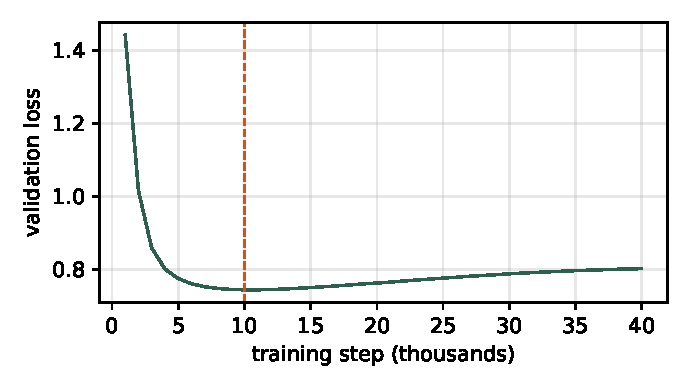
\includegraphics[width=0.6\linewidth]{generated/latent_lm_val.pdf}
\caption{From-scratch latent LM: validation loss rises after 10k steps (dashed).}
\label{fig:lm}
\end{figure}

\subsection{Negative and weak results: automatic quality measures}

\paragraph{Friction-noise measure.} The listener's most frequent complaint was ``sawing'': left-hand friction
noise that is idiomatic in moderation but grating when overused. A measure of noisy high-band frames correlated
with the score in the wrong direction (Spearman $\rho=+0.39$ over 48 clips), and the nine clips tagged as
sawing had \emph{lower} noisy-frame fractions than the rest (0.0006 vs 0.0017).

\paragraph{Pentatonic fit.} The fraction of tonal energy on the best-fitting pentatonic set tracked scores over
124 rated clips ($\rho=0.52$, positive in each study) but only weakly among candidates for the same opening
($\rho=0.31$ after removing group means). Choosing the best-fitting candidate raised the mean from 3.41 to 3.52;
discarding the worst raised it to 3.58. Restricting the measure to pitches at note onsets---motivated by the
listener's observation that idiomatic semitones occur in slides, not at the pluck---was weaker still
($\rho_{\text{within}}=0.19$), although generated clips did place more onsets outside the mode than real recordings
(33\% vs a median of 22\%; 39\% in clips flagged for semitones). The measure on its own also disagreed with R5,
where it predicted that longer training worsened modal fit while the listener preferred the longer-trained
model.

\subsection{Rater consistency}

Fifteen clips from R6 were rated again, unknowingly, in R7. Six scores were identical, twelve within one point,
and the mean absolute difference was 0.8. A clip chosen for the showcase in one session received a 1 in the next
when heard next to an alternative. Context effects of this size are comparable to the differences between our
models and are the main reason we do not claim significance.

\section{Long playback by chained continuation}\label{sec:chain}

To extend the favourite 35\,s clip, we repeatedly fed its last 15\,s as an opening and appended 30\,s of new
material. Two problems appeared.

\paragraph{Silent tails.} Every generated clip ends with about 0.5\,s of digital silence ($-87$\,dBFS) as the
requested duration runs out. When that tail is part of the next opening, the model treats the piece as ended and
inserts a further two seconds of silence at the seam. Trimming the source's last 1.5\,s and over-generating each
segment by 3\,s, then discarding the tail, removed the gaps.

\paragraph{Loudness feedback.} Each segment came out slightly louder than its opening, and that segment became the
next opening: over six rounds the level rose from $-10$ to $-5.5$\,dBFS with up to 10\% of samples clipped. Feeding
every opening at a fixed level ($-16$\,dBFS) and matching each new segment to the level of the 15\,s before it kept
the 3.5-minute result between $-13.8$ and $-16.7$\,dBFS per 30\,s with no clipping. Of two locked chains, the listener accepted one
and rejected the other for a sudden breakdown after 82\,s, a reminder that long-range stability is not solved.

\section{Limitations and ethics}\label{sec:limits}

\paragraph{Evaluation.} All ratings come from one listener, who is also the author and designed the systems; the
studies are small and were run sequentially as development proceeded, so later studies are not independent of
earlier decisions. In R2 the openings came from a performer who, contrary to the original plan, had been included
in the 412-recording training set. Multi-listener studies, objective measures validated against them, and checks
for replication of training material~\citep{batlleroca2024replication} are needed before stronger claims.

\paragraph{Data and rights.} The training recordings are commercially published historical performances and are
not redistributed; we do not release the adapter weights. We release code, the listening ratings and the
analysis that produces every number in this report \todo{repository URL}. The base model is used under
Stability AI's community license. Openly licensed guqin recordings we could find amount to under one hour.

\paragraph{Cultural context.} The narratives and tags are our condensed readings of traditional notes on each
piece and simplify a rich interpretive tradition; 22 of the 108 titles are inferred from the title alone.

\section{Conclusion}

A pretrained latent diffusion model, a few tens of hours of carefully screened historical recordings, a small
adapter and a single attentive listener were enough to produce guqin continuations and scene-driven pieces that
the listener rated highly, while training a generator from scratch on the same data failed completely. The
strongest effects were not from architecture but from data curation, held-out early stopping, and simple
engineering of the generation loop. The next steps are multi-listener evaluation, preference-based fine-tuning
on the collected ratings~\citep{wallace2023diffusiondpo}, and stable long-form generation for continuous playback.

\section*{Acknowledgements}
Code for data processing, training orchestration, evaluation pages and analysis was written with the help of
AI coding assistants (OpenAI Codex and Anthropic Claude); all experimental decisions and all listening judgements
are the author's. \todo{other acknowledgements}

\bibliographystyle{plainnat}
\bibliography{references}

\end{document}
